\chapter{Introduction}\label{introduction}
//TODO Write what is NLP

\chapter{Dialogue systems}\label{dialogue systems}
Dialogue system is a computer system to communicate with a human. Nowadays you meet dialog systems everywhere. A lot of devices have incorporated goal-oriented spoken dialogue systems, such as  Yandex’s Alisa,  Apple’s Siri, Microsoft’s Cortana, Amazon Alexa, and Google Assistant. Dialogue systems are also used in cars (hands-free car-specific functions, Android Auto, Apple CarPlay, vendor-specific solutions), web (search assistants (IKEA), Facebook Messenger and Telegram chatbots), robots, computer games, research systems (skylar.speech.cs.cmu.edu) etc, because a conversation is a natural way for people to get information.

\textbf{Basic Dialogue System Types}:
\begin{itemize}
  \item Task-oriented 
    \begin{itemize}
      \item focused on completing a certain task(s)
    \end{itemize}
  \item Non-task-oriented
    \begin{itemize}
      \item chitchat
      \item gaming the Turing test
    \end{itemize}    
\end{itemize}

\textbf{Communication Domains}:

"\textbf{Domain}" is a conversation topic or an area of interest
\begin{itemize}
  \item Single/Closed-domain is one well-defined area
  \item Multi-domain is joining several single-domain systems
  \item Open-domain “responds to anything”
\end{itemize}


Exists several \textbf{modes of communication}:
\begin{itemize}
  \item Text
  \item Voice
  \item Multimodal
    \begin{itemize}
      \item voice/text + graphics
      \item additional modalities: video - gestures, mimics; touch
    \end{itemize}
\end{itemize}

\textbf{Dialogue initiative}:
\begin{itemize}
  \item system-initiative
    \begin{itemize}
      \item system asks questions, user must reply in oreder to progress
      \item least natural
      \item "form-filling" ("Hello, please enter your e-mail") 
    \end{itemize}
  \item user-initiative
    \begin{itemize}
      \item user asks, machine responds ("Siri, set the timer for 5 minutes")
    \end{itemize}
  \item mixed-initiative
    \begin{itemize}
      \item system and user both can ask and react to queries
      \item most natural
    \end{itemize}
\end{itemize}

\textbf{Dialogue system architecture} is illustrated in Figure \ref{ds architecture}. This architecture consists from Natural Language Understanding (NLU), dialogue management (DM), and Natural Language Generation (NLG).

\textbf{NLU} extracts the meaning from the user utterance and converts into a structured semantic representation. Natural Language Understanding traditionally consists of domain identification and intent prediction, which are framed as utterance classification problems, and slot filling, framed as a sequence tagging task.

\textbf{DM} plays two roles,tracking the dialogue state and performing the dialogue policy (i.e., telling the agent how to act given the dialogue state.)

\textbf{NLG} transforms structured data into natural language.\cite{open_domain_neural_ds}
\begin{figure}[hbt]
  \centering
  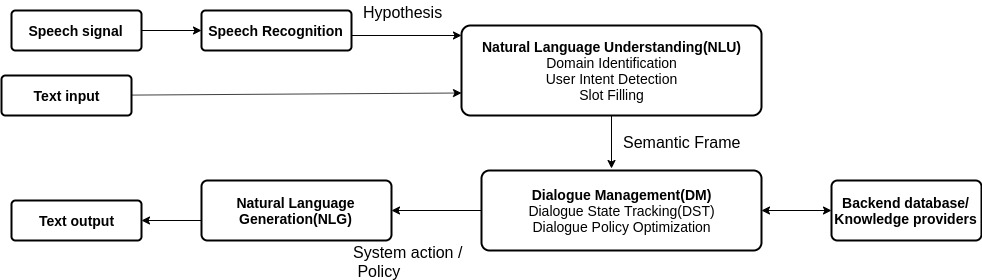
\includegraphics[width=0.8\textwidth]{figures/ds_arcitecture.jpg}
  \caption{Dialogue system architecture.}
  \label{ds architecture}
\end{figure}

\chapter{Natural Language Generation}\label{nlg}
Natural Language Generation is a subsection of Natural Language Processing (NLP). 
NLG approaches can be grouped into two categories, one focuses on generating text using templates or rules (linguistic) methods, the other uses corpus-based statistical methods, where \textbf{corpus} is a collection of texts.

\subsection*{Categories of Natural Language Generation approaches}

\textbf{Template-based} systems map their non-linguistic input directly to the linguistic surface structure. This linguistic structure may contain gaps. Well-formed outputs does not cointain gaps.
The template-based system selects a proper response for the current conversation from a repository with response selection algorithms. 

\textbf{Advantages:}
\begin{itemize}
  \item Robust and reliable
  \item The output produced by this modules is likely to be grammatically correct and not contain unexpected generation errors
  \item Generation process is fully controlles
\end{itemize}

\textbf{Disadvantages:}
\begin{itemize}
  \item Number of templates grows quickly (different templates for singular and plural versions)
  \item Expensive and time-consuming to deploy a real dialogue system
  \item Limits its usage to other domains
  \item Not much variation in output (no planning of text; simple concatenation of strings)
  \item Not able to handle unknown inputs 
  \item Templates often sound unnatural due to their generic structures
  \item Not able to learn and not able to adapt to the user
\end{itemize}

\begin{center}
\textbf{Example}: "The 306 train leaves Aberdeen at 11:20 am"

\vspace{5mm}
Semantic representation: 

$Departure(train_{306}, location_{abdn}, time_{1120})$

\vspace{5mm}
Template: 

[train] \textit{is leaving} [town] \textit{now}
\end{center}
The gaps represented by \textbf{[train]} and \textbf{[town]} are filled by looking up the relevant
information in a table. More information you can find in \cite{applied_nlg}.

In \textbf{corpus-based} systems it is possible directly mimicking the language of a real domain expert, rather than attempting to model it by rule and this category is able to generate more proper responses that could have never appeared in the coprus, but a good corpus is necessary. 
\cite{stochastic_language_generation_ds} \cite{survey_on_ds}

\subsection*{NLG problems}
The NLG component converts an abstract dialogue action into natural language surface utterances. As noticed in \cite{generator_problems}, a good generator usually relies on several factors: adequacy (similarity in meaning), fluency (syntactic correctness), readability (efficacy in context), and variation.

\chapter{Other}
Oh and Rudnicky showed that stochastic generation benefits from two factors: 
\begin{itemize}
  \item it takes advantage of the practical language of a domain expert instead of the developer
  \item it restates the problem in terms of classification and labeling, where expertise is not required for developing a rule-based generation system
\end{itemize}

Non-task-oriented dialogue system

The aim of task-oriented dialogue systems is to complete specific tasks fo user, non-task-oriented dialogue systems focus on conversing with human on open domains. 

//TODO: more information in article []
//TODO: Info about datasets
//TODO: NLP vs Computation linguistic

//TODO: In non task oriented dialogue systems it is very difficult to use template-based generation
\cite{stochastic_language_generation_ds}
